% CHAPTER two -- global trait compilation

\section*{Keywords}
Terrestrial vertebrates; traits; coverage; completeness; taxonomic biases; spatial biases; phylogenetic biases.

\section*{Abstract}
Trait data are increasingly used in studies investigating the impacts of global changes on the structure and functioning of ecological communities. Despite a growing number of trait data collations for terrestrial vertebrates, there is to date no global assessment of the gaps and biases the data present. Here, I assess whether terrestrial vertebrate trait data are taxonomically, spatially and phylogenetically biased. I compile seven ecological traits and quantify coverage as the proportion of species for which an estimate is available. For a species, I define completeness as the proportion of non-missing values across traits. I assess whether coverage and completeness differ across classes and examine phylogenetic biases in trait data. To investigate spatial biases, I test whether wider-ranging species have more complete trait data than narrow-ranging species. Additionally, I test whether species-rich regions, which are of most concern for conservation, are less well-sampled than species-poor regions.
My results show that mammals and birds are well-sampled even in species-rich regions. For reptiles and amphibians (herptiles), only body size presents a high coverage (>80\%), as well as habitat related variables (for amphibians). Herptiles are poorly sampled for other traits. The shortfalls are particularly acute in some species-rich regions and for certain clades. Across all classes, geographically rarer species have less complete trait information. Hence, trait information is less available on average in some of the most diverse areas and in geographically rarer species, both critical for biodiversity conservation. Gaps in trait data may impede our ability to conduct large scale analyses, while biases can impact the validity of extrapolations. A short-term solution to the problem is to estimate missing trait data using imputation techniques, while a longer-term and more robust filling of existing gaps requires continued data collection efforts.

\section{Introduction}
Species traits are fundamental to ecological and evolutionary research. Comparative studies regularly use trait data across organisms to understand evolutionary processes and species coexistence \citep{Escudero2016, Zamudio2016}, to investigate global patterns of life forms and functions \citep{Diaz2016}, or to assess species’ vulnerability to environmental changes \citep{Bohm2016, Pacifici2015, Pearson2014}. Because traits influence species’ ability to cope with environmental changes \citep{Newbold2013} and underpin species’ contributions to ecosystem processes \citep{Lavorel2002a, Violle2007, Wong2018}, they play an increasingly important role in functional and conservation ecology.

Past and recent efforts to collate and release trait data in the public domain have facilitated the development of trait-based research. For instance, a global trait database has been published for plants \citep{Kattge2011}. As of May 2020, data from this database had been used in 297 publications since its release (Activity report, 18/06/2020, \url{https://www.try-db.org/TryWeb/Home.php}). Such databases hence constitute invaluable research tools and have the potential to greatly advance the field.

Vertebrates are one of the most studied taxa \citep{Titley2017}. There are now diverse sources of ecological traits for vertebrate groups (primates: \cite{Galan-Acedo2019}; mammals: `PanTHERIA', \cite{Jones2009}; amniotes: \cite{Myhrvold2015}; amphibians: ‘AmphiBIO’, \cite{Oliveira2017}). These datasets stem from important efforts to collate published estimates of trait data and make them readily available. Trait data have also been made available on online platforms (for instance, the Global Assessment of Reptile Distribution initiative: \url{http://www.gardinitiative.org/}; the IUCN Red List of Threatened Species: \url{https://www.iucnredlist.org/}; BirdLife data zone: \url{http://datazone.birdlife.org/home}).

Nevertheless, despite the importance of vertebrate species in global research outputs, there is no single source for vertebrate ecological traits. Consequently, researchers wishing to conduct comparative studies across vertebrate groups may have to collate trait data from a range of sources (such as in \citet{Cooke2019a, Cooke2019b} or in \citet{Gonzalez2018}), a time-consuming prerequisite which may be a limiting step of the research process. Indeed, collating data from heterogeneously-formatted sources presents many challenges \citep{Schneider2019}, particularly when working across a large number of species. For instance, traits may be measured differently across datasets; units may be inconsistent; and taxonomic resolution and nomenclature may vary.

The lack of a curated, readily available global database for vertebrate ecological traits impedes our ability to conduct cross-taxon comparative studies at global scales. However, efforts to collate data into a single database are limited by the availability of underlying data. Because there exist important gaps in biodiversity knowledge \citep{Hortal2015}, trait datasets are often incomplete, with many species lacking estimates for many traits. The incompleteness of ecological trait data at the species level has been termed the `Raunki{\ae}ran shortfall' by \citet{Hortal2015}. Furthermore, incomplete trait data are likely to be biased. Biases in trait data may be the consequence of uneven taxonomic and spatial collection effort, with a set of charismatic or easily detectable species being more completely sampled. For instance, \citet{Gonzalez-Suarez2012} investigated biases in global trait information in mammals. They notably found that the availability of mammalian trait data was geographically and phylogenetically biased, with larger and more widely distributed species being better sampled. In addition, data availability also differed across IUCN Red List extinction risk categories, with threatened species (Critically Endangered, Endangered or Vulnerable) being less well sampled for traits than non-threatened species (Least Concern or Near Threatened).

A major issue with incomplete, biased data is the introduction of bias in subsequent analyses. Assessing the amount of missing data as well as the so-called ‘missingness mechanism’-- whether missing data are missing at random, as opposed to there being systematic biases in the way missing values are distributed, see \citet{Baraldi2010} -- is an important prerequisite. Indeed, there exist diverse techniques to deal with data missingness. The simplest one consists of retaining complete cases only by filtering out missing values (case deletion, see \citet{Nakagawa2008}). Nevertheless, case deletion may lead to biased parameter estimates and erroneous conclusions when values are not missing at random \citep{Gonzalez-Suarez2012}. Therefore, it is critical to determine the most appropriate way to deal with data incompleteness. For instance, previous studies using terrestrial vertebrate trait data have employed multiple imputation techniques to fill in the gaps \citep{Gonzalez-Suarez2012, Cooke2019b}. Yet, imputation techniques could be sensitive to non-randomness in trait data. Phylogenetic biases (where some clades are under-sampled compared to other clades) could notably impact the performance of several imputation approaches. It is thus vital to characterise the gaps in trait data prior to any analysis. However, there has been no study to date investigating global patterns in the availability of trait data across terrestrial vertebrates.

Here, I aim to assess the global state of trait data in terrestrial vertebrates. I focus on a set of traits that are available across the four classes and that are commonly used by ecologists: body size; litter or clutch size; longevity; trophic level; activity time; habitat breath; and a measure of habitat specialisation. I quantify and compare the gaps in trait data across classes by calculating the coverage of each trait across species, and the completeness of trait estimates for each species (Box 1). I investigate taxonomic, spatial and phylogenetic biases in trait coverage and completeness.

Given that biodiversity research is globally biased towards birds and mammals \citep{Titley2017}, I hypothesise that herptiles are less well sampled for traits than mammals and birds, having both lower coverage and completeness.

Furthermore, building upon previous studies conducted on mammals \citep{Gonzalez-Suarez2012}, I hypothesize that species rarity influences completeness, focusing on species geographical range size as one aspect of rarity. Widely distributed species could be better sampled than narrowly distributed species because their ranges overlap with more study sites, regardless of their abundance. As such, I test whether species geographical range size explains trait completeness. 

It is well established that global research effort is distributed unequally \citep{ONU2015}, with patterns underpinned by various geographical and socioeconomic factors. For instance, countries with higher gross domestic product tend to host a larger number of research institutions \citep{Martin2012}. The proximity of research infrastructures and the accessibility of survey sites play an important part in explaining the global distribution of knowledge \citep{Hortal2015}. As a result of these factors, biodiversity data gaps tend to be greater in tropical areas \citep{Collen2008}. Tropical areas have the greatest species richness, and so these data biases are of great concern for biodiversity conservation. Whether species-rich regions are systematically under-sampled for traits compared to species-poor regions is thus important to assess, given the significance of species-rich areas for global conservation. Here, I investigate spatial biases in trait completeness, hypothesizing that species-rich areas are on average less well sampled than species-poor areas.

Finally, I investigate phylogenetic biases in the trait data. I assess whether particular clades have received more attention than others by looking for patterns in the distribution of trait completeness across the terminal branches of phylogenetic trees in each class.

\clearpage

\begin{mdframed}
\label{Trait_definition_box}
\textbf{Box 1. Definitions}\\
\textit{Trait:} Sensu stricto, a characteristic measurable at the level of an individual and that influences organismal fitness or performance \citep{Violle2007}. In this thesis, I broaden this definition to include `ecological' traits (e.g., the number of habitats used by a species), where the relationship of a species to the surrounding environment needs to be considered. Ecological traits may be estimated by aggregating data across multiple individuals.\\
\textit{Trait completeness:} For a given species, the proportion of traits for which an estimate is available.\\
\textit{Trait coverage:} For a given trait, the proportion of species for which an estimate is available.
\end{mdframed}


\section{Methods}

I produced class-specific trait datasets that were made available on figshare (DOI: \url{10.6084/m9.figshare.10075421}).
Data compilation and all analyses were conducted with R version 3.5.1 \citep{R_citation}.
Distribution maps were processed using both R and the ArcPy package available in ArcGIS v.10.6 \citep{ESRI} (implemented in Python 2.7; \citet{Python_citation}).

\subsection{Trait data collection}

\subsubsection{Sources and taxonomic matching}

I used freely accessible secondary sources in my compilation (Table \ref{datasources}), selected for their broad taxonomic coverage and/or for their frequent use in macroecological studies. Across sources, similar species could appear under synonymic names. This was a potential problem for matching sources by binomial names. Indeed, synonymy can artefactually decrease trait coverage, when trait information is not available across all synonyms. Notably, difficulties arise when species have been divided into several subspecies or when different subspecies are clumped together. Systematic manual checks could not be applied considering the scale of the data collection (there were $>$39,000 unique binomial names across sources). I developed a procedure aiming at identifying one accepted name for each of the binomial names found across sources. When I could not find an accepted name, I used the original name. Figure \ref{chart_taxcor} summarizes the main steps; similar solutions have been used in other large-scale studies \citep{Cooke2019b}.

Briefly, the procedure consisted of extracting synonyms from the IUCN \citep{IUCN2020} or from the Integrated Taxonomic Information System (ITIS; \url{https://www.itis.gov/}), using the rredlist \citep{rredlist} and taxize \citep{Chamberlain2013} R packages. One accepted name was assigned to each synonym. I produced a “Synonym” dataset that I have also made available. I then normalized taxonomy across sources by replacing binomial names with their identified accepted name where applicable.

Given that different taxonomic backbones could be used to correct for taxonomy, I make two versions of the trait compilations available (corrected and not corrected for taxonomy), meaning that users are free to apply their own corrections; for example, taxonomy could be aligned to that of class-specific sources, such as The Reptile Database, the American Museum of Natural History’s Amphibian Species of the World, the Mammal Diversity Database or the International Ornithological Congress World Bird List. Datasets corrected for taxonomy contain 11,634 species of birds, 5,381 mammals, 10,612 reptiles and 6,990 amphibians. Where no taxonomic correction was applied when matching sources, the compiled datasets contain 13,501 birds, 5,791 mammals, 11,012 reptiles and 8,583 amphibians. For more information, see Appendix 2 (S2.1; Figure \ref{SI2_taxcor}).

%%%%%%%%%%%%%%%%%%%%%%%%%%%%%%%%%%%%%%%%%%%%%%%%%%%%%%%%%%%%%%%%%%%%%
%% figure 1: procedure for taxonomic checks
\vskip 1cm
\begin{figure}[h!]
\centering
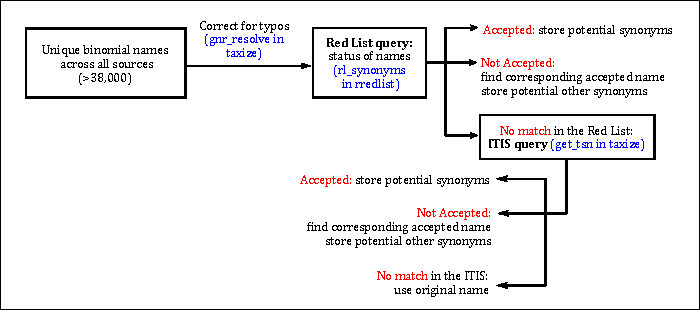
\includegraphics[scale=1.4]{figures/Chapter2/Taxonomic_corrections_chart}
\caption[Procedure used to identify the accepted names of species]{\textbf{Procedure used to identify the accepted names of species.} I extracted, where possible, the accepted names of species from either the IUCN Red List or the Integrated Taxonomic Information System (ITIS). \textit{Figure reproduced from \citet{Etard2020}.}}
\label{chart_taxcor}
\end{figure}


%%%%%%%%%%%%%%%%%%%%%%%%%%%%%%%%%%%%%%%%%%%%%%%%%%%%%%%%%%%%%%%%%%%%%
%% table with references for trait data
\begin{table}[h!]
\renewcommand{\baselinestretch}{1}
\renewcommand{\arraystretch}{1.5}
\begin{center}\fontsize{9}{11}\selectfont
\caption[Data sources for each trait]{\textbf{Data sources for each trait.} Abbreviations: A = amphibians; B = birds; BL = body length; BM = body mass; DA = diel activity time; GL = generation length; H = habitat data; LCS = litter or clutch size; L/ML = longevity or maximum longevity; M = mammals; MA = age at sexual maturity; R = reptiles; RS = range size; TL = trophic level. Note. Data sources may contain more traits than shown here. Tick marks in parentheses indicate that the trait was present in the data source but that another closely related trait with a better coverage was used instead. The tilde character ($\sim$) before a tick mark indicates that I derived trophic levels from species diet. $^1$ \url{http://datazone.birdlife.org/home}; $^2$ \url{https://www.iucnredlist.org/resources/spatial-data-download}; $^{3}$\url{http://apiv3.iucnredlist.org/api/v3/docs$\#$general}. \textit{Table reproduced from \citet{Etard2020}.}} 
\label{datasources}
\begin{tabular}{|l|c|c|c|c|c|c|c|c|c|c|c|}
\hline
\multicolumn{1}{|c|}{\multirow{2}{*}{\textbf{Sources}}} & \multirow{2}{*}{\textbf{Taxa}} & \multicolumn{10}{c|}{\textbf{Traits}}                                                                                                       \\ \cline{3-12} 
\multicolumn{1}{|c|}{}                                  &                                & \textbf{BM} & \textbf{BL} & \textbf{L/ML} & \textbf{MA} & \textbf{GL} & \textbf{LCS} & \textbf{TL} & \textbf{DA} & \textbf{RS} & \textbf{H} \\ \hline
\citet{Oliveira2017}                                                & \multirow{4}{*}{Amphibians}    & (\checkmark )         & \checkmark            & (\checkmark )           & \checkmark            &             & \checkmark             & $\sim$\checkmark           & \checkmark            &             &            \\ \cline{1-1} \cline{3-12} 
\citet{Cooper2008}                                                  &                                &             &             &               &             &             & \checkmark             &             &             &             &            \\ \cline{1-1} \cline{3-12} \begin{comment}
\textit{Senior dataset}$^1$                                                  &                                &             & \checkmark            &               &             &             &              &             &             &             &            \\ \cline{1-1} \cline{3-12} \end{comment}
\citet{Sodhi2008}                                                   &                                &             & \checkmark            &               &             &             &              &             &             &             &            \\ \hline
\citet{Wilman2014}                                                  & \multirow{2}{*}{Birds}         & \checkmark            &             &               &             &             &              & $\sim$\checkmark           & \checkmark            &             &            \\ \cline{1-1} \cline{3-12} 
BirdLife$^1$                                                &                                & \checkmark            &             &               &             & \checkmark            &              &             &             &    \checkmark         &            \\ \hline
\citet{Jones2009}                                                   & \multirow{5}{*}{Mammals}       & \checkmark            & (\checkmark )         & (\checkmark )           & (\checkmark )         &             & \checkmark             &             & \checkmark            &             &            \\ \cline{1-1} \cline{3-12} 
\citet{Kissling2014}                                                &                                &             &             &               &             &             &              & \checkmark            &             &             &            \\ \cline{1-1} \cline{3-12} 
\citet{Gainsbury2018}                                               &                                &             &             &               &             &             &              & \checkmark            &             &             &            \\ \cline{1-1} \cline{3-12} 
\citet{Wilman2014}                                                   &                                & \checkmark            &             &               &             &             &              &             & \checkmark            &             &            \\ \cline{1-1} \cline{3-12} 
\citet{Pacifici2015}                                                 &                                & \checkmark            &             &          &        & \checkmark            &              &             &             &             &            \\ \hline
\citet{Scharf2015}                                                  & \multirow{10}{*}{Reptiles}      & \checkmark            &             & \checkmark              & (\checkmark )         &             & \checkmark             & \checkmark            & \checkmark            &             &            \\ \cline{1-1} \cline{3-12} 
\citet{Vidan2017}                                                   &                                &             &             &               &             &             &              &             & \checkmark            &             &            \\ \cline{1-1} \cline{3-12} 
\citet{Stark2018}                                                   &                                & \checkmark            &             & \checkmark              &             &             & \checkmark             &             & \checkmark            &             &            \\ \cline{1-1} \cline{3-12} 
\citet{Schwarz2017}                                                 &                                &             &             &               &             &             & \checkmark             &             &             &             &            \\ \cline{1-1} \cline{3-12} 
\citet{Novosolov2017}                                        &                                & \checkmark            &             &               &             &             &              & \checkmark            &             &             &            \\ \cline{1-1} \cline{3-12} 
\citet{Novosolov2013}                                         &                                &             &             &               &             &             & \checkmark             &             &             &             &            \\ \cline{1-1} \cline{3-12} 
\citet{Slavenko2016}                                            &                                & \checkmark            &             &               &             &             &              &             &             &             &            \\ \cline{1-1} \cline{3-12}
\citet{FeldmanGEB2016}                                            &                                & \checkmark            &             &               &             &             &              &             &             &             &            \\ \cline{1-1} \cline{3-12}
\citet{Meiri2018GEB}                                            &                                &            &             &               &       \checkmark       &             &       \checkmark        &     \checkmark         & \checkmark             &             &            \\ \cline{1-1} \cline{3-12}
\citet{Meiri2015}                                            &                                &             &             &               &             &             &              &       \checkmark                         &         \checkmark                       &      &            \\ \cline{1-1} \cline{3-12}
\citet{Roll2017}                                            &                                &             &             &               &             &             &              &                                &      & \checkmark       &           \\ \hline
\citet{Myhrvold2015}                                         & B, M, R      & \checkmark            & \checkmark            & \checkmark              & (\checkmark )         &             & \checkmark             &             &             &             &            \\\hline \cline{1-1} \cline{3-12} 
\citet{IUCN2020} $^{2}$                                           &            A, B, M                   &             &             &               &             &             &              &             &             & \checkmark             &  \\ \hline
\citet{IUCN2020} $^{3}$                                           &        All                         &             &             &               &             &             &              &             &             &             & \checkmark           \\ \hline

\end{tabular}
\end{center}
\end{table}

%%%%%%%%%%%%%%%%%%%%%%%%%%%%%%%%%%%%%%%%%%%%%%%%%%%%%%%%%%%%%%
%%%%%%%%%%%%%%%%%%%%%%%%%%%%%%%%%%%%%%%%%%%%%%%%%%%%%%%%%%%%%%




\subsubsection{Compilation methods}
For continuous traits, I took the median value within species when multiple estimates were available from different sources, after removal of any repeated values, which were assumed to represent estimates duplicated across secondary compilations and derived from the same underlying primary sources. Although intraspecific variation is increasingly being recognized to have important effects on ecological systems \citep{Bolnick2011, Siefert2015, DesRoches2018, GonzalezSuarez2012a}, it was not feasible to obtain measures of intraspecific variability from all sources; therefore, estimates were provided as a single measure for each species. For some species and some traits, measures were provided separately for females and males. In such cases, I first obtained the mean of these two measures.

Across sources, there were multiple traits related to each of body size and life span. For instance, body mass and/or body length information could be provided. Different proxies were also available for life span, such as the age at sexual maturity or generation length. In such cases, I focused on the trait presenting the highest coverage.

\begin{itemize}
\item \textbf{Body size}\\
Adult body mass estimates were compiled for mammals, birds and reptiles. Body length information was compiled for amphibians, because the coverage for body length was higher than that for body mass. Body mass and body length are known to scale allometrically, although the allometric relationship differs across amphibian clades \citep{Santini2018}. In the amphibian dataset, Pearson’s correlation coefficient between log(Body mass) and log(Body length) was 0.71 (data points shown in Appendix 2, S2.2, Figure \ref{SI2_amphibians}).
 
\item \textbf{Longevity}\\
I defined longevity as the life span of an individual and maximum longevity as the longest life span reported. I used closely related traits when longevity/maximum longevity was not available or when longevity/maximum longevity had a poorer coverage than a related trait. I selected the age at sexual maturity for amphibians; Pearson’s correlation coefficient between log(Age at sexual maturity) and log(Maximum longevity) was 0.55 (Appendix 2, S2.2, Figure \ref{SI2_amphibians}). I compiled the generation length for mammals and birds. The correlation between log(Generation length) and log(Longevity) was 0.74 for mammals and 0.70 for birds (data points shown in Appendix 2, S2.2, Figure \ref{SI2_birdsmammals}). Finally, I used maximum longevity directly for reptiles.

\item \textbf{Litter or clutch size}\\
The number of offspring (litter size) or eggs (clutch size) was compiled directly from the sources and treated as equivalent across classes. I reported measures of central tendencies provided by the sources where applicable; otherwise, I calculated range midpoints (mean of smallest and largest reported litter/clutch sizes).

\item \textbf{Trophic level}\\
In all classes, species were described as omnivores, carnivores or herbivores. For reptiles and mammals, this information was compiled directly from the sources. For amphibians and birds, trophic levels were not provided. For these two classes, I inferred trophic levels from dietary information (Table \ref{datasources}). For birds, I used the primary diet (based on food items recorded as composing $\geq$50\% of the diet of a species). Diet for amphibians was described without respect to the percentage use of food items; simply as a binary record of whether or not food items were used. In both cases, species recorded to only consume plant-based resources (seeds, nectar, fruit or other plant material) were classified as herbivores. Species consuming only animal resources (invertebrates or vertebrates) were classified as carnivores. Species consuming a mixture of plant and animal resources were classified as omnivores.

\item \textbf{Activity time}\\
Species were described as being either nocturnal or non-nocturnal. Despite a higher resolution of activity time information in some of the sources (e.g., species being described as cathemeral, crepuscular or diurnal), I adopted the classification of the source with the lowest resolution (EltonTraits: \citet{Wilman2014}, for birds), in order to have consistent information across classes. As such, all species defined as diurnal, cathemeral or crepuscular were classified as non-nocturnal, as opposed to species classified as strictly nocturnal.

\item \textbf{Habitat breadth}\\
I used IUCN habitat data \citep{IUCN2020}, which describe species habitat preferences and the suitability and importance of each habitat. I defined habitat breadth as the number of habitats a species was known to use, using level 2 of the IUCN Habitat Classification Scheme for description of habitat types (divided into: Forest, Savanna, Shrubland, Grassland, Wetland, Rocky areas, Caves and subterranean, Desert, Marine, Marine intertidal or coastal/supratidal, Artificial, Introduced vegetation, and Other/Unknown.) Note that the total number of habitats, determined by including those that qualify as artificial, correlates positively with the number of natural habitats used (Figure \ref{Fig_HB_main}).

%% figure habitat breadth
\begin{figure}[h!]
\centering
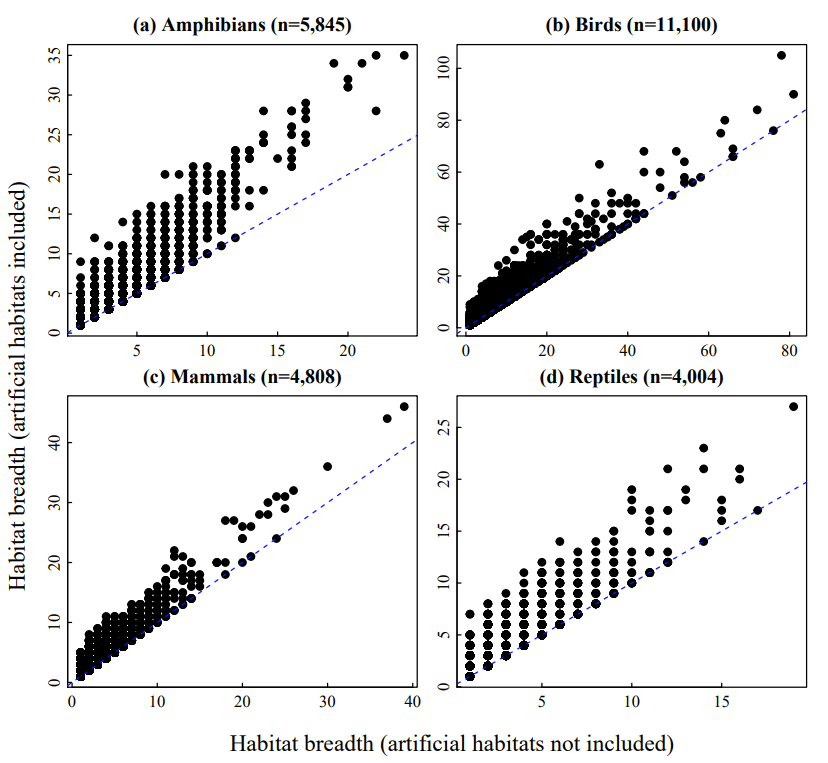
\includegraphics[scale=0.7]{figures/Chapter2/Fig_HB_main}
\caption[Number of natural and artificial habitats used by a species against number of strictly natural habitats used by a species]{\textbf{Number of natural and artificial habitats used by a species against number of strictly natural habitats used by a species}. Pearson's correlation coefficients show a high positive correlation between these two metrics of habitat breadth in all terrestrial vertebrate classes: 0.92 for amphibians \textbf{(a)}, 0.95 for birds \textbf{(b)}, 0.94 for mammals \textbf{(c)}, and 0.90 for reptiles \textbf{(d)}.}
\label{Fig_HB_main}
\end{figure}


\item \textbf{Use of artificial habitats}\\
For a species, I recorded whether any artificial habitat was reported to be suitable in the IUCN habitat data.
\end{itemize}

Finally, the compiled datasets contain an additional column, `Note', where I reported species found to be extinct or extinct in the wild (EW). I used species Red List status and information from \citet{Meiri2018GEB} to flag such species. I reported 75 extinct/EW species for mammals, 160 for birds, 34 for amphibians and 53 for reptiles. It is likely that the datasets contain extinct species that I could not flag, because they were not recorded as extinct in the sources I used.

\newpage
\subsubsection{Phylogenies}
I used class-specific phylogenetic trees downloaded on 13 April 2020. For mammals, I used `complete' trees from \citet{Faurby2018, Faurby2020}, downloaded from \url{https://zenodo.org/record/3690867#.Xyc5wyhKhPZ}. For amphibians, birds and squamates, I obtained trees from \url{https://data.vertlife.org/}. The original sources were as follows: \citet{Jetz2012} for birds; \citet{Jetz2018} for amphibians; and \citet{Tonini2016} for squamates. For each class, a distribution of 1,000 trees was available. For plotting purposes, I obtained consensus trees using the TreeAnnotator program of the BEAST software \citep{Bouckaert2019}.

\subsubsection{Species distributions}
I obtained extent-of-occurrence distribution maps for reptiles from \citet{Roll2017}, available at: \url{https://datadryad.org/stash/dataset/doi:10.5061/dryad.83s7k} (downloaded 13 April 2020). For mammals and amphibians, species distribution maps were obtained from the IUCN Red List (\citet{IUCN2020}, downloaded 13 April 2020); for birds, they were obtained from BirdLife International (\url{http://datazone.birdlife.org/species/requestdis}, downloaded 17 April 2020).

For amphibians, mammals and birds, I selected areas of extant or probably extant presence only. Additionally, I selected areas where species were resident or present during the breeding season, and I excluded areas occupied during the non-breeding season or where species were considered vagrant.

In addition, for all classes, I excluded occupied areas that fell outside the known elevational limits of species, where such data were available. Lower and upper elevational limits were retrieved from the IUCN Red List (queried using the rredlist package) and were available for approximately half of the species (Supporting Information, Appendix 2, S2.3, Figure \ref{SI2_elev_limits}). Decreases in range sizes were observed after cutting distribution maps by the known elevational limits (Appendix 2, S2.3, Figure \ref{SI2_cutalt_ranges}).

\subsection{Investigating gaps and biases in trait data}

I used trait coverage and completeness to investigate taxonomic, phylogenetic and spatial biases in the trait data. Table \ref{Chap1_samplesizes} summarizes the sample sizes (number of species) in each of the following analyses. Note that species for which completeness was 0\% were included in all analyses (for more details, see Figure \ref{1_Coverage}). Also note that I did not filter out species identified as extinct or extinct in the wild, because they represented a small proportion of the datasets (0.48\% for amphibians, 1.4\% for both birds and mammals, and 0.50\% for reptiles) and also because I could not exclude such species systematically, because it is likely that I did not flag them all.

%%%%%%%%%%%%%%%%%%%%%%%%%%%%%%%%%%%%%%%%%%%%%%%%%%%%%%%%%%%%%%
%%%%%%%%%%%%%%%%%%%%%%%%%%%%%%%%%%%%%%%%%%%%%%%%%%%%%%%%%%%%%%
\vskip 0.5cm

%  Table 2 sample sizes
\begin{table}[!htbp] 
\renewcommand{\baselinestretch}{1}
\renewcommand{\arraystretch}{1.5}
\begin{center}\fontsize{9}{11}\selectfont
\caption[Number of species for each analysis]{\textbf{Number of species for each analysis.} All species represented in the trait datasets were included in (1). All species from the class-specific phylogenetic trees or from the distribution maps that matched with species in the trait datasets were included in (2) and (3). \textit{Table reproduced from \citet{Etard2020}.}}
\label{Chap1_samplesizes}
\begin{tabular}{@{\extracolsep{5pt}} cccc} 
\\[-1.8ex]\hline 
\hline \\[-1.8ex]  & \textbf{(1) Taxonomic biases} & \textbf{(2) Phylogenetic biases} & \textbf{(3) Spatial biases} \\ 
\hline \\[-1.8ex] Amphibians & $6,990$ & $6,170$ & $5,650$ \\ 
Birds & $11,634$ & $8,315$ & $10,802$ \\ 
Mammals & $5,381$ & $5,171$ & $5,046$ \\ 
Reptiles & $10,612$ & $9,404$ & $9,382$\\
\hline \\[-1.8ex] 
\end{tabular} 
\end{center} 
\end{table} 
%%%%%%%%%%%%%%%%%%%%%%%%%%%%%%%%%%%%%%%%%%%%%%%%%%%%%%%%%%%%%%
%%%%%%%%%%%%%%%%%%%%%%%%%%%%%%%%%%%%%%%%%%%%%%%%%%%%%%%%%%%%%%


\subsubsection{Taxonomic biases}
I tested whether completeness varied across taxonomic class using pairwise Wilcoxon rank sum tests. I tested for the extent and performance of the taxonomic corrections by looking at trait coverage when taxonomic corrections are applied and when no correction is applied (Appendix 2, S2.4, Figure \ref{SI_2_deltaCov_taxcor}).

\subsubsection{Phylogenetic biases}
Initially, to assess whether more closely related species were more likely to be similar in trait completeness, I estimated the phylogenetic signal in completeness with Pagel’s $\lambda$ \citep{Pagel1999} in each class. I used a bootstrapping approach, calculating $\lambda$ for each of 50 trees randomly sampled in each class (using the phylosig function of the phytools R package; \cite{Revell2012}). I then estimated the mean and 95\% confidence intervals (95\% CIs) of $\lambda$. Sample sizes for computing $\lambda$ (number of species represented in both the phylogenies and trait datasets) are shown in Table \ref{Chap1_samplesizes}.

I then plotted within-family median completeness in phylogenetic trees built at the family level, using the consensus trees. Within-family median completeness was calculated using taxonomic information in the trait datasets (sample sizes shown in Table \ref{Chap1_samplesizes}).

\subsubsection{Spatial biases}

I first investigated whether wider-ranging species were more likely to be better sampled than narrow-ranging species. I tested for a relationship between species range size and trait completeness. I fitted a generalized linear model with a Poisson error distribution (directly using the number of sampled traits, `N\textsubscript{traits}', rather than the proportion (completeness)). Class was added as a predictor interacting with range size; thus the model was:
\begin{center}
N\textsubscript{traits} $\sim$ log(Range size) $\ast$ Class. 
\end{center}
Second, I mapped assemblage-level median completeness. Assemblages were characterized at the pixel level at 50 km$^2$ resolution. I determined pixel-level composition and richness by stacking species geographical distributions. I then calculated median completeness across species in each pixel. I show the resulting maps for herptiles in the main text, and for mammals and birds in Appendix 2 (S2.5, Figure \ref{SI2_mediancomp_spatial}; median completeness was very high across most pixels for mammals and birds). In addition, I provide maps of assemblage-level mean completeness and standard deviation for all classes in Appendix 2 (S2.5; Figures \ref{SI2_meancomp_spatial} and \ref{SI2_sdcomp_spatial} show corresponding maps; Figure \ref{SI2_sdcomp_sr} shows standard deviation against species richness).

I then tested for a spatial correlation between species richness and median completeness. Given that median completeness was very high across most pixels for mammals and birds, I fitted such models for herptiles only. I fitted spatial autoregressive lag models to explain assemblage-level median completeness as a function of species richness (using the function lagsarlm of the spatialreg package \citep{spatialreg1, spatialreg2, spatialreg3}). Given that responses could vary geographically, I included the biogeographical realm as an interacting factor (using the World Wide Fund for Nature (WWF) ecoregion shapefile to characterise realms, obtained from \url{https://www.worldwildlife.org/publications/terrestrial-ecoregions-of-the-world}); the considered realms were Afrotropics, Australasia, Indo-Malayan, Nearctic, Neotropics and Palaearctic. To improve normality, I arc-sin square-root transformed completeness values and log-transformed species richness. The lagsarlm function allows for a consideration of spatial autocorrelation in the dependent variable by estimating the autoregressive lag coefficient, $\rho$, associated with an n-by-n matrix of spatial weights, \textit{W}. The final model was:
\begin{center}
$\arcsin(\sqrt{\text{Completeness}})\sim \log(\text{Species richness}) \ast \text{realm} + \rho \cdot W \cdot \arcsin(\sqrt{\text{Completeness}})$.\\
\end{center}

The value of \textit{W} was estimated using the functions tri2nb and nb2listw of the spdep package \citep{spatialreg3, spdep1}. Fitting the model using all grid cells was computationally intractable; therefore, I randomly sampled cells for this analysis (using 30\% of the grid cells in each realm). I selected grid cells where species richness was higher than three to avoid sampling issues. I fitted separate models for amphibians and reptiles, because when adding class as an interacting predictor, the same cells (with the same coordinates) might be sampled for multiple classes, whereas the tri2nb function does not tolerate duplicated coordinates.

\section{Results}

\subsection{Taxonomic biases in trait information}
Trait coverage for mammals and birds was overall high (Figure \ref{1_Coverage}(a); mean and median coverage across traits: 89\% and 95\% for mammals; 84\% and 85\% for birds). In both cases, litter/clutch size was the trait with the poorest coverage (61\% for mammals and 59\% for birds). Coverage exceeded 80\% for all other traits (except  trophic level for birds, at 75\% coverage).

Conversely, trait coverage was more variable for herptiles, and poorer overall (Figure \ref{1_Coverage}(a); mean and median trait coverage: 47\% and 32\% for amphibians, 46\% and 38\% for reptiles). Coverage exceeded 80\% only for body size in both reptiles and amphibians and for habitat related traits in amphibians only. In all other cases coverage was  $<$55\%, with very little information available for longevity--related traits. 

Trait completeness (proportion of non-missing trait values for a species) reflected similar biases (Figure \ref{1_Coverage}(b)). The distribution of trait completeness varied significantly among classes (pairwise Wilcoxon rank sum test: p--value$<$0.0001 in all cases). Distributions were highly left skewed in mammals and birds (skewness: -2 and -1.6). 84\% of all mammalian species and 80\% of avian species fell in the 80--100\% completeness range. Moreover, the completeness distribution was moderately right skewed for reptiles (skewness: 0.4), and slightly right skewed for amphibians (skewness: 0.02). 56\% of all reptiles and 57\% of amphibians fell in the 0-50\% completeness range. 

\begin{figure}[h!]
\centering
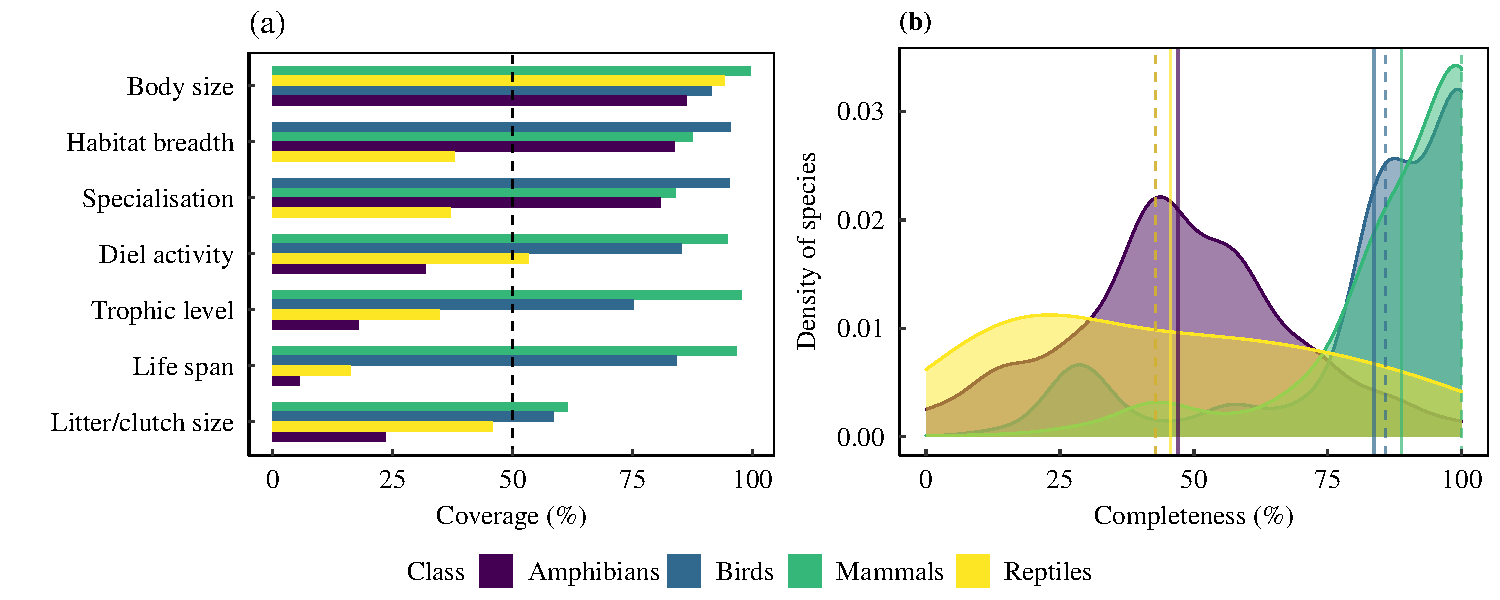
\includegraphics[scale=0.7]{figures/Chapter2/Figure1_revised}
\caption[Trait coverage and completeness across species]{\textbf{Trait coverage and completeness across species.} \textbf{(a)} I defined coverage as the proportion of species for which an estimate is available for a given trait. The dashed line represents 50\% coverage. \textbf{(b)} Trait completeness is the proportion of estimated traits for a species. Here, I show the distribution of completeness. Continuous lines represent the mean trait completeness for each class, whereas dashed lines represent the median trait completeness. Note that there were species with 0\% completeness (230 species for amphibians -- 3.3\% of amphibian species in the trait dataset; 9 for birds -- 0.077\% of species; 7 for mammals -- 0.13\% of species; and 161 for reptiles -- 1.5\% of species). Species with 0\% completeness were retained in the datasets when there was information for traits I did not select in the analyses, but no known value for the traits I did select. For instance, the body mass of the amphibian species \textit{Rhinella centralis} was known, but other trait values (including body length) were missing, meaning that \textit{Rhinella centralis} had 0\% completeness for the set of traits I considered. \textit{Figure reproduced from \citet{Etard2020}.}}
\label{1_Coverage}
\end{figure}


\subsection{Phylogenetic biases in trait completeness}
As expected from the distribution of trait completeness in mammals and birds (Figure \ref{1_Coverage}), within-family median trait completeness was high across most tips of the phylogenetic trees (Appendix 2, Figures \ref{SI2_phymammals} and \ref{SI2_phybirds}; I present the avian and mammalian phylogenies in the Appendix because there was little variation in completeness across tips). For birds, $\lambda$ was 0.71 ($\pm$ 0.0053). For mammals, $\lambda$ was 0.78 ($\pm$ 0.0035). This indicated that, despite completeness generally being high across tips, the sampling was not evenly distributed across the phylogeny.

In herptiles, clusters of families with similar median trait completeness appeared (Figure \ref{1_Phylo}). In amphibians, groups of families belonging to the order Anura (frogs) showed both the best and worst median completeness (Figure \ref{1_Phylo}(a)). The best-sampled families included the tailed frogs of the family Ascaphidae (two species) and species of the family Leiopelmatidae (four species endemic to New Zealand). The family Ceratobatrachidae (containing \textit{c.} 90 species occurring in Southeast Asia and in some Pacific islands), the family Ranidae (true frogs, 450 species considered here) and the family Rhacophoridae (shrub frogs, 382 species considered here) figured among the worst-sampled families. For amphibians, $\lambda$ was 0.63 ($\pm$ 0.0039). In reptiles, most snakes were poorly sampled, whereas families in other suborders appeared to be sampled better overall (Figure \ref{1_Phylo}(b)). Within snakes, the pythons, boas, the three species of the family Acrochordidae and the python-like species of the family Loxocemidae were better sampled than other snake families. In reptiles, $\lambda$ was 0.69 ($\pm$ 0.0032). The sampling in herptiles was thus also uneven with regard to the phylogeny.

It is important to underline that Figure \ref{1_Phylo} shows within-family median completeness, masking the considerable variation in species richness across families, hence masking potential important variation in completeness across species within families. For example, in the amphibian family Allophrynidae (three recognized species), the within-family median completeness was 50\%; but the dataset comprised two species of completeness 14\% and 86\%, respectively. I present similar plots to those in Figure \ref{1_Phylo} showing the within-family standard deviation in completeness in Appendix 2 (Figure \ref{SI2_sd_phylo_herptiles}). Within-family standard deviation tended to increase with within-family species richness (Appendix 2, Figure \ref{SI2_sd_sr_herptiles}).

\clearpage

\begin{figure}[h!]
\centering
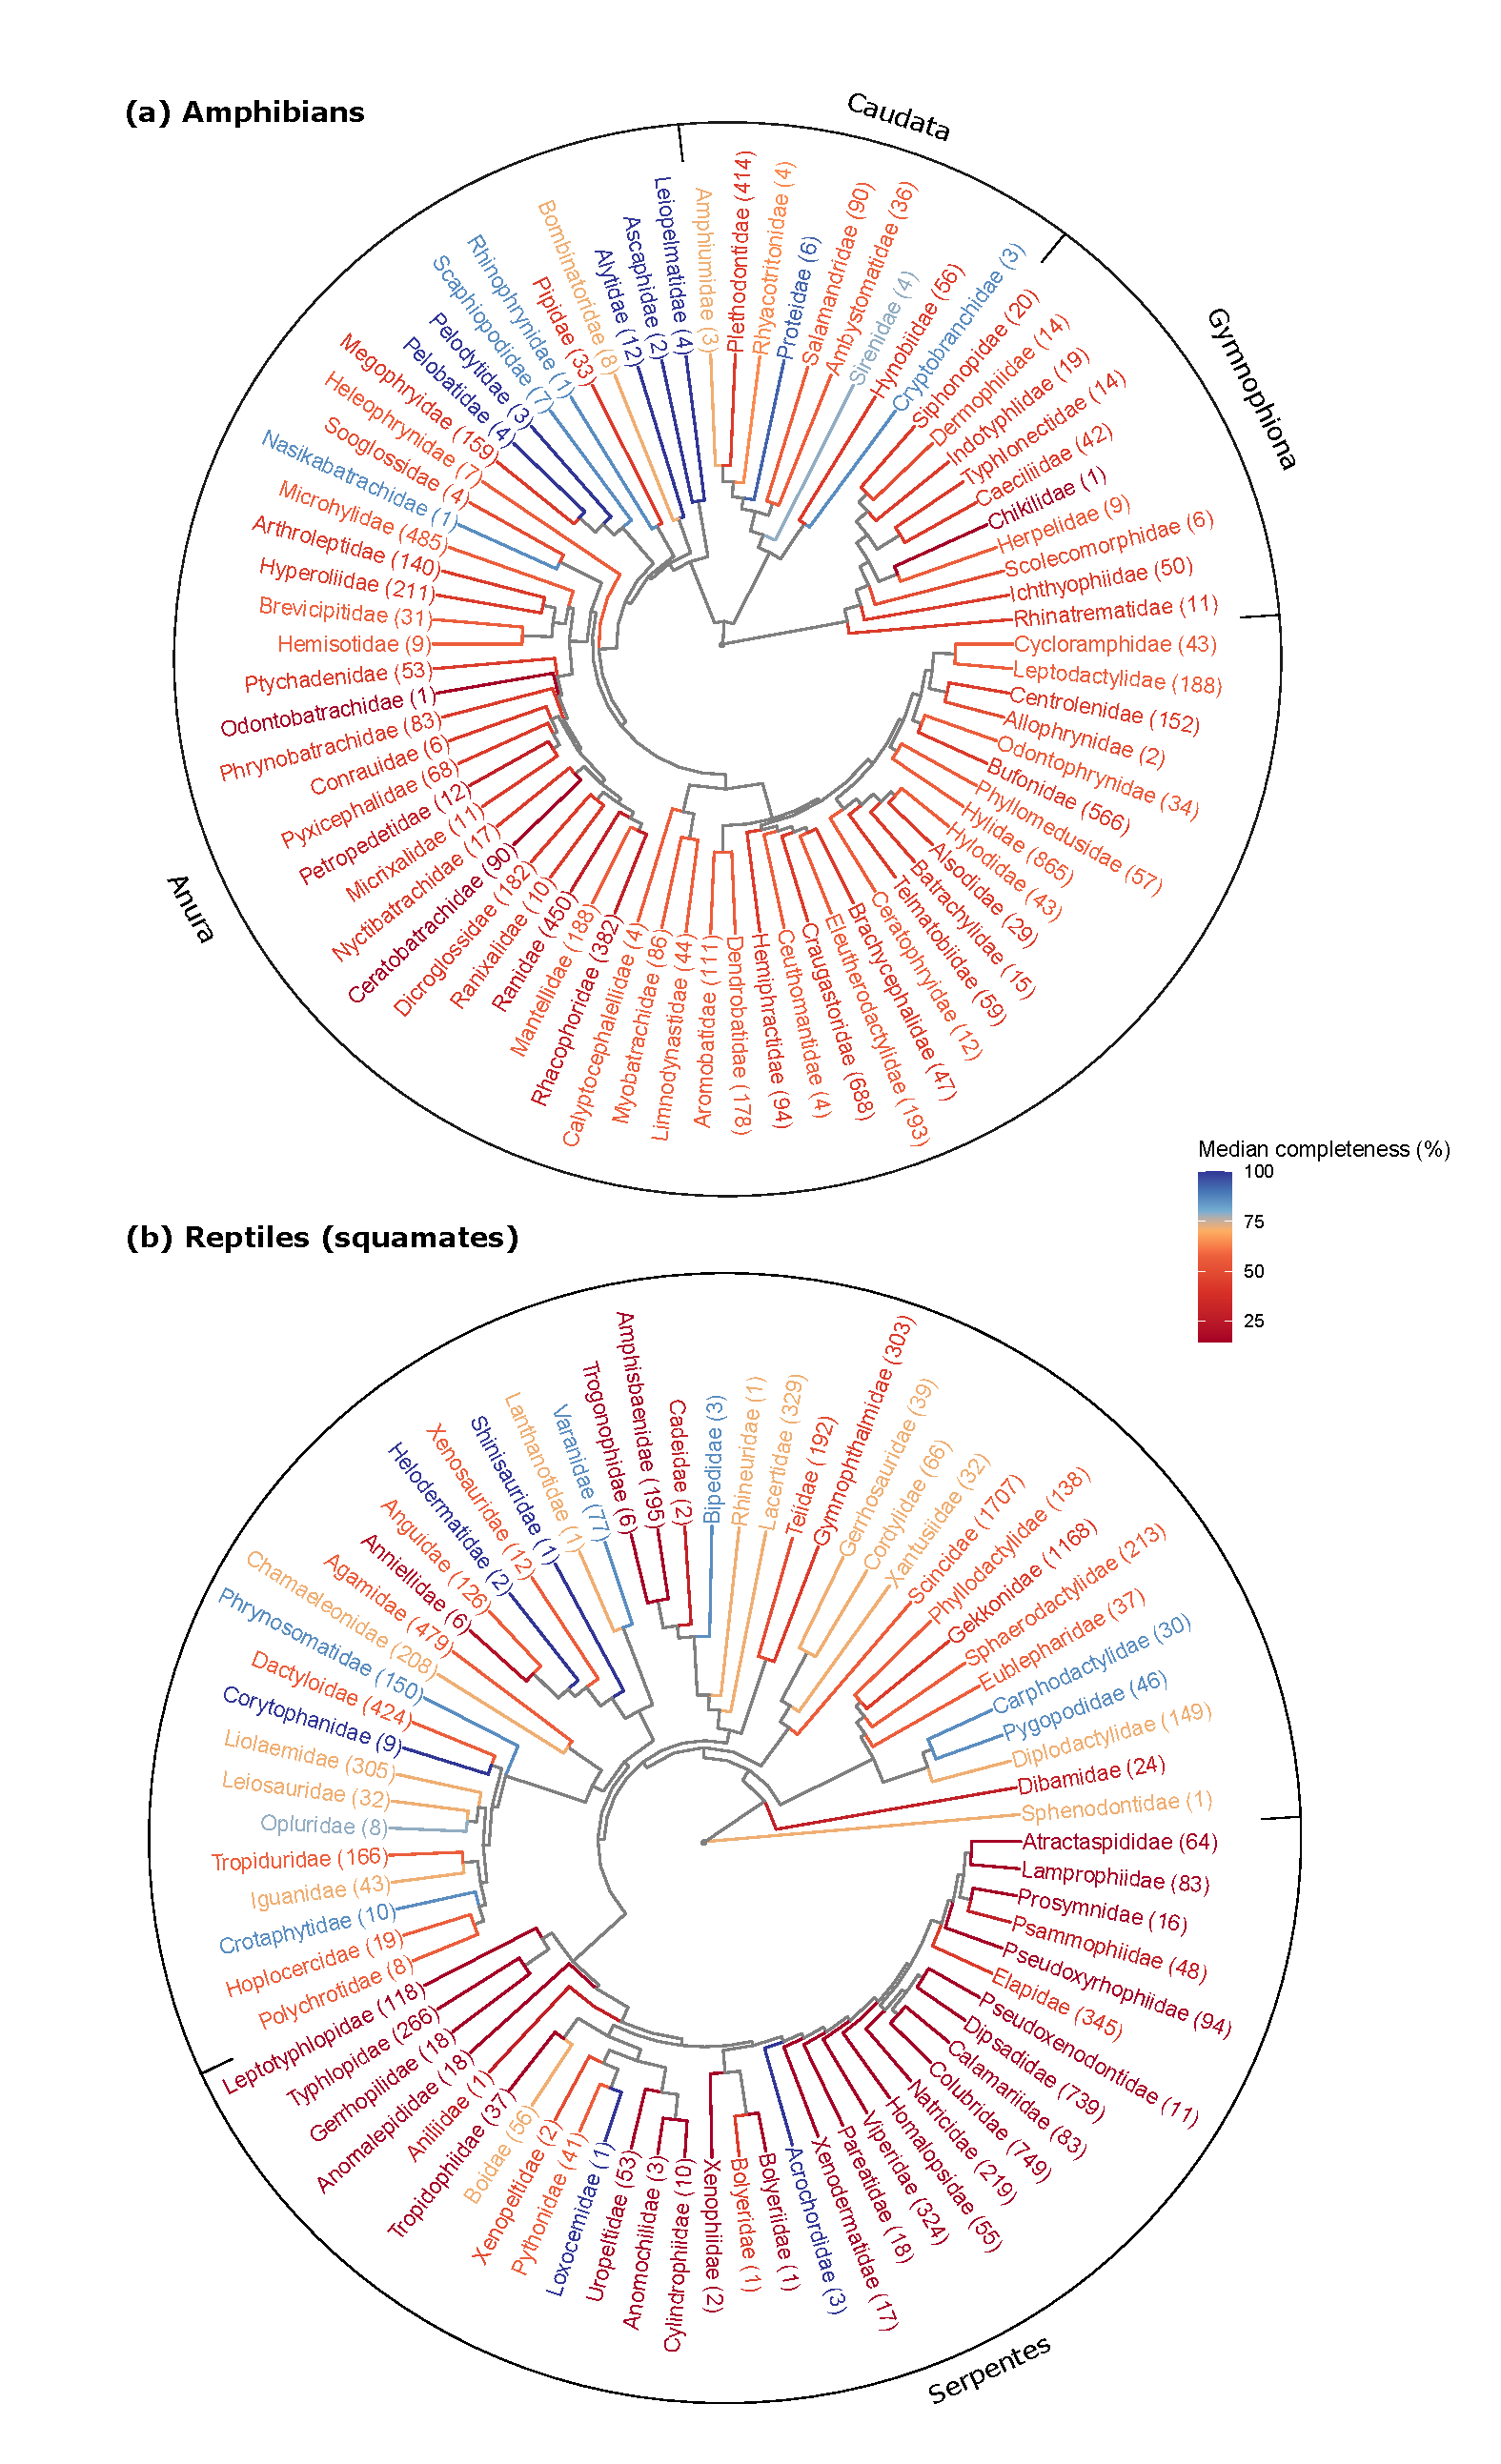
\includegraphics[scale=0.5]{figures/Chapter2/Figure_3}
\caption[Within-family median trait completeness in herptiles]{\textbf{Within-family median trait completeness in herptiles.} The number next to each family name represents the number of species included in the calculation of the median. \textit{Figure reproduced from \citet{Etard2020}.}}
\label{1_Phylo}
\end{figure}

\clearpage

%% pick up the referencing to the SI figures here

\subsection{Spatial biases in trait completeness}
Range size was significantly correlated with the number of sampled traits. Larger range sizes were associated with a higher number of sampled traits (i.e., with higher completeness; Figure \ref{1_Range_size}; Appendix 2, S2.7, Table \ref{SI2_summary_RS}). Similar results were obtained when using distribution maps not cut by elevational limits (Appendix 2, S2.7, Table \ref{SI2_summary_RS_notcut}; Figure \ref{SI2_plot_RS_notcut}). The rate of increase was steepest for reptiles, then for amphibians, then for birds and mammals (slope estimates for birds and mammals were not significantly different from each other; Appendix 2, Table \ref{SI2_summary_RS}).

\begin{figure}[h!]
\centering
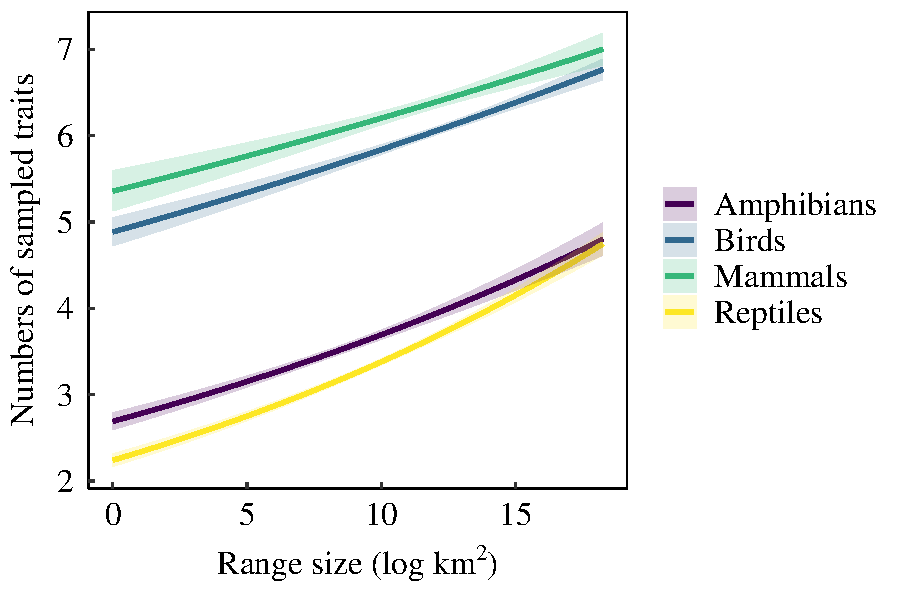
\includegraphics[scale=0.7]{figures/Chapter2/Figure_4}
\caption[Relationship between number of sampled traits and geographical range size]{\textbf{Relationship between number of sampled traits and geographical range size.} Models were fitted using a Poisson error distribution. Class was added as a predictor interacting with range size. Rates of increase in number of sampled traits with range size were not significantly different for mammals and birds but differed for reptiles and amphibians, with the steepest rates of increase for reptiles. \textit{Figure reproduced from \citet{Etard2020}.}}
\label{1_Range_size}
\end{figure}

There were marked spatial variations in median trait completeness in herptiles (Figure \ref{2_Map}). North America and Europe were well sampled for both amphibians and reptiles. Moreover, Southeast Asia and the Congo basin were on average less well sampled. In other regions, contrasting patterns emerged between amphibians and reptiles. For instance, median completeness was poorer for amphibians than for reptiles in Australia, but opposite patterns were observed in South America. As in the phylogenetic analyses, assemblage-level median completeness could mask potential important variation in completeness within species of a given assemblage. Assemblage-level mean and standard deviation maps are shown in Appendix 2 (S2.5, Figures \ref{SI2_meancomp_spatial} and \ref{SI2_sdcomp_spatial}). There was a trend for increasing standard deviation with increasing species richness, with a larger spread in standard deviation at lower species richness (Appendix 2, section S2.5, Figure \ref{SI2_sdcomp_sr}).

\clearpage

\begin{figure}[h!]
\centering
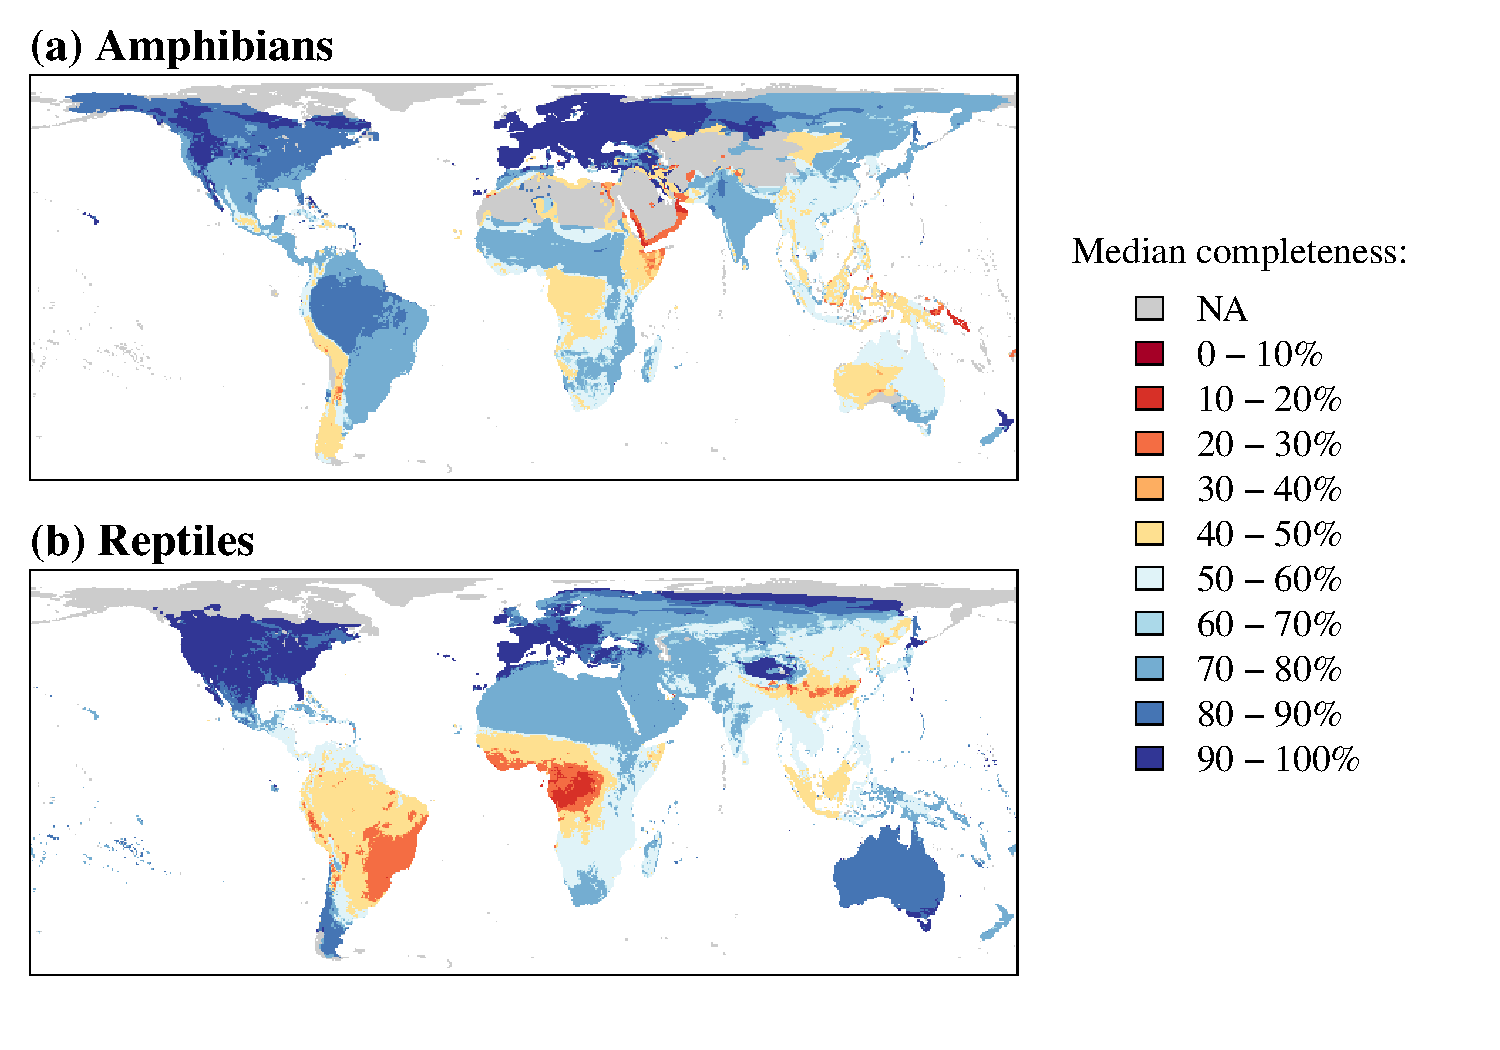
\includegraphics[scale=0.7]{figures/Chapter2/Figure_5}
\caption[Spatial distribution of assemblage-level median trait completeness in herptiles]{\textbf{Spatial distribution of assemblage-level median trait completeness in herptiles.} Similar maps for birds and mammals are shown in Appendix 2 (S2.5, Figure \ref{SI2_mediancomp_spatial}). \textit{Figure reproduced from \citet{Etard2020}.}}
\label{2_Map}
\end{figure}


Spatial models showed that species richness explained median trait completeness in herptiles in most realms (Figure \ref{2_Trends}; Appendix 2, S2.8, Tables \ref{SI2_summary_spatial_amphibians} and \ref{SI2_summary_spatial_reptiles}); including spatial lags improved the models (amphibians: $\rho$ = 0.92, p-value < 0.0001; reptiles: $\rho$ = 0.91, p-value < 0.0001). For reptiles, completeness was negatively correlated with species richness in the most species-rich realms (Afrotropics, Indo-Malayan and Neotropics) and in the Palaearctic; the relationship was steepest in the Afrotropics and shallowest in the Palaearctic. In the Australasian and Nearctic realms, completeness tended to increase with species richness. For amphibians, negative relationships were observed in the Indo-Malay and Nearctic realms, whereas positive trends were observed in the Neotropics and the Palaearctic. The opposite trends between reptiles and amphibians observed in the Australasian and Neotropical realms reflected patterns observed on the maps. The Indo-Malayan was the only realm where median completeness tended to decrease with species richness for both reptiles and amphibians.

\clearpage
\begin{figure}[h!]
\centering
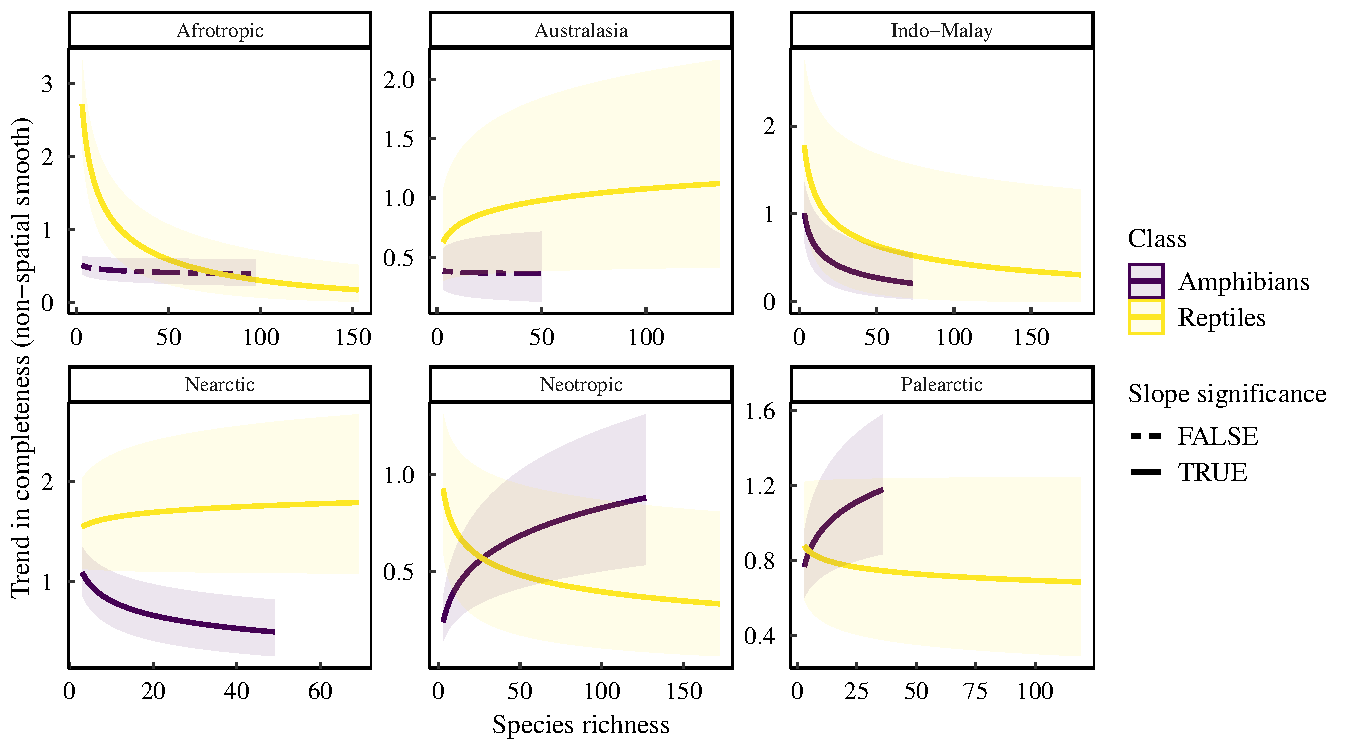
\includegraphics[scale=0.75]{figures/Chapter2/Figure_6}
\caption[Spatial model trends for herptiles]{\textbf{Spatial model trends for herptiles.} The lines represent in-sample predictions ($\pm$ standard error) for the trend components of the spatial models (trends after accounting for spatial autocorrelation). \textit{Figure reproduced from \citet{Etard2020}.}}
\label{2_Trends}
\end{figure}


\section{Discussion}

The results of this Chapter illustrate the taxonomic, spatial and phylogenetic dimensions of the knowledge gaps in trait data, termed the Raunkiæran shortfall by \citet{Hortal2015}. To the best of my knowledge, this work constitutes the first comparative assessment of global gaps for terrestrial vertebrate trait data, despite their use in numerous studies. I showed that the trait data present important taxonomic, spatial and phylogenetic biases, with contrasts in the availability of trait information between, on the one hand, herptiles and, on the other hand, birds and mammals.

Birds and mammals are globally well sampled for the set of traits I considered, even in the most species-rich assemblages. Moreover, the availability of trait information for herptiles is lower overall and phylogenetically and geographically biased. Several factors could interplay to shape these patterns. For instance, species that are more easily detectable (for example, wider ranging) and more charismatic are likely to be better sampled. Diverse socio-economic predictors could also contribute to geographical biases in trait data sampling; global biases in primary data collection are likely to be one of the most important contributors to the patterns I highlighted. Nevertheless, biases in the data could have been introduced at later stages, notably with the selection of sources and traits. The global compilation I obtained in this chapter reflects, in part, the interest and focus of the secondary data sources I used. It is possible that the addition of new sources from regional journals or other authorities could diminish spatial biases in the data by increasing coverage for certain areas. Nevertheless, I argue that by focusing on widely used traits, these results are likely to reflect the “true” availability of the data in primary sources and that the shortfalls for other, less used traits would be more pronounced.

I believe that the results presented here are robust to taxonomic uncertainty, although taxonomic matching might potentially be improved further using class-specific sources, such as the Reptile Database or AmphibiaWeb, for identification of synonyms (but see Appendix 2, S2.9, Figure \ref{SI2_taxcor_rangebuilder}). I have made two versions of the data compilations available, one in which my own corrections were applied and one using the original binomial names of the sources, meaning that users are free to use their own taxonomic backbones and identify synonyms within the compilations.
I believe that taxonomic matching is a recurring issue when working across thousands of species. Taxonomic synonymy artefactually inflates the numbers of identified species, potentially lowering trait coverage (whereas clumping subspecies together can have the opposite effect). Tackling this problem is difficult \citep{Isaac2004, Jones2012}, notably because there is no global curated database recording the status of species names, and also because of the nature of taxonomy and the debates around the species concept \citep{May2011}. Nevertheless, taxonomic uncertainty can have important consequences. For instance, \citet{Cardoso2017} showed that inaccuracies and errors in species checklists contributed to the overestimation of plant diversity in the Amazon (but see \citet{Freeman2021}: the relative underdescription of species in tropical areas compared to temperate  areas --`taxonomic debt', also referred to as `latitudinal taxonomic gradient' by the authors-- may lead to the underestimation of species richness at low latitudes).

Biases in trait data have important implications for conservation planning. Past studies have shown that narrow-ranged species, for which fewer trait data are available on average, have higher extinction risks \citep{Collen2016, Purvis2000, Ripple2017} and are more negatively impacted by anthropogenic pressures than wider-ranging species \citep{Newbold2018a}. Trait information is also less available for herptiles in tropical regions such as the Congo basin, Southeast Asia and South America, which are some of the most diverse areas of crucial importance for worldwide conservation \citep{Barlow2018}. Consequently, trait information is on average less available where potentially more crucial to conservation planning. Indeed, trait information can be incorporated into vulnerability assessments and, as such, can help to prioritize conservation efforts. Species traits have been found to mediate species responses to environmental changes across diverse taxonomic groups, and thus can inform on the sensitivity of species to anthropogenic pressures \citep{Flynn2009, Newbold2013, Nowakowski2017}. Traits are now commonly used to estimate species vulnerability or extinction risks \citep{Pacifici2015, RamirezBautista2020}. As opposed to trend-based approaches, which rely on historical population trends (changes in abundance or shifts in distributions) to predict species’ vulnerability and extinction risks, trait-based approaches rely on species’ intrinsic sensitivity to particular threats. The appeal of trait-based approaches to extinction risk estimation is that, by providing mechanistic insights, they diminish the amount of population information needed. If the responses of species to a threat consistently relate to certain traits, it is possible to generalize patterns across species for which population data are less available \citep{Verberk2013}. Integrating traits into vulnerability assessments is hence of particular interest when field monitoring of species population sizes or distributions is difficult to achieve, but biases in the data could mean that such information is lacking for some of the most vulnerable species.

%% 

Traits that influence species responses to environmental changes have been termed `response traits' (or `response-mediating traits'; \citet{Luck2012}), as opposed to `effect traits' that underpin ecosystem functioning \citep{Lavorel2002a}. For instance, relative brain size and longevity have been characterized as response traits in birds \citep{Newbold2013, Sayol2020}, whereas dietary characteristics (e.g., trophic levels or guilds) are both response and effect traits. \citet{Hortal2015} highlighted that, for plants, both response and effect traits have been investigated, whereas for vertebrates the research has been more focused on understanding species responses. This could be because the way vertebrate traits interact to shape some ecosystem processes has not yet been characterized well.

Ecosystem processes sustained by animals might be harder to quantify and might be influenced by a combination of traits. The traits compiled in this work are likely to have a role in diverse processes. Nevertheless, there was one important omission, in that I did not compile species diet in this chapter, potentially the most straightforward trait to link with diverse processes, such as grazing, pollination, scavenging and seed dispersal. From a practical perspective, I chose traits that had been estimated at least for some of the species in each class, and that were readily available. Diet was excluded because although estimates were available for amphibians, birds and mammals, there was no readily available database for reptilian diet. Movement or dispersal abilities were also excluded because information was not readily available for any class. Although I expect that species diet and dispersal abilities would present similar sampling biases to the ones presented in this work, the addition of such traits to the compilation would represent a valuable contribution and would notably facilitate studies looking at the functional roles of reptiles.

For practical reasons, I did not consider intraspecific trait variation. Intraspecific variation has been shown to have important effects on ecological systems, and a growing body of literature encourages trait-based research to include intraspecific variability \citep{Guralnick2016}. There have been several calls to produce open-access, global trait datasets \citep{Weiss2019}, including a representation of intraspecific trait variation \citep{Kissling2018}. Notably, \citet{Schneider2019} designed a framework to store and share inter- and intraspecific trait data, accompanied by an R package to standardize the data in a proposed format. Such a proposition could constitute an important step towards the unification of individual datasets into a single, comprehensive database for ecological trait data.

The current spatial and taxonomic gaps in trait data might limit our ability to scale studies up, whereas biases in the data can affect the validity of extrapolations to groups or areas that are undersampled. More generally, biases and gaps in biodiversity data can have important implications for ecological studies. Data gaps can hinder our ability to draw conclusions on observed macroecological patterns. For example, \citet{CHAUDHARY2016} proposed that marine species richness follows a bimodal distribution, peaking at mid-latitudinal locations, and argued that these patterns were not underpinned by knowledge gaps in species distributions. Nevertheless, \citet{Menegotto2018} attributed the tropical dip in marine species richness to a lack of species distribution data, explained by lower sampling efforts in tropical areas (`Wallacean' shortfall; \citet{Hortal2015}). Biases and gaps in trait data could also affect studies in closely related fields, such as functional ecology -- for instance, past studies have shown that functional diversity indices are sensitive to missing data \citep{Majekova2016, Pakeman2014} -- or community assembly \citep{Perronne2017}.

Ecologists should, therefore, take particular care when designing trait-based studies, because both data quality and data gaps are likely to influence the results and the generality of the conclusions. There exist diverse methods to deal with missing trait values, should data missingness be problematic. Complete removal of missing values (`case deletion') is commonly used but presents several issues, because it reduces sample size and statistical power and introduces potential bias in data subsamples \citep{Nakagawa2008}. For example, retaining complete cases only from the trait datasets would generate trait data disproportionally representative of mammals and birds, which would be problematic for conducting cross-taxon analysis on terrestrial vertebrates. As such, it is recommended that case deletion be applied only when data are missing completely at random, which is rarely the case \citep{Peugh2004}.

Alternatives to case deletion consist of filling in the gaps. In recent years, the development of imputation techniques has provided robust methods to handle missing data. Such imputation techniques have been used to complete trait datasets in recent studies \citep{Cooke2019b}. \citet{Penone2014} used a simulation approach to evaluate the performance of four of these techniques, namely PhyloPars \citep{Bruggeman2009}, random forest algorithms as implemented in R with missForest \citep{Stekhoven2016, Stekhoven2012}, multivariate imputation by chained equations (MICE; \citet{micepackage}) and k-nearest neighbour (kNN; \citet{Troyanskaya2001}). \citet{Penone2014} introduced missing values (10\%–80\%) in a complete trait dataset of carnivorans and measured imputation performance in different scenarios. Given that phylogenetic non-randomness in missing trait values can impact imputation accuracy, \citet{Penone2014} removed values in three different ways (completely at random; with a phylogenetic bias; and with a body mass bias). Out of the four techniques, missForest and PhyloPars performed best when species phylogenetic position was included as a predictor of missing trait values. Such imputations appeared to be robust even when trait coverage was as low as 40\%, which might be relevant for many reptilian and amphibian traits. The performance was not significantly affected by phylogenetic non-randomness of the data. Hence, missForest and PhyloPars appear to be well suited when traits are phylogenetically conserved, because they allow species phylogenetic position to be included as a predictor of missing trait values. The study by \citet{Penone2014} highlights that there are robust imputation techniques allowing to deal with incomplete trait data where biases might otherwise be problematic. Nevertheless, it is important to highlight that some imputation techniques, such as single or mean imputation, can be problematic because they do not allow an estimation of uncertainty and suffer from a lack of accuracy \citep{Nakagawa2008}; indeed, imputation techniques sometimes perform no better than case deletion. More work should be conducted to assess imputation performance in various contexts (see Johnson 2021), and the datasets compiled in this chapter might provide an opportunity for such studies.

%% Add Johnson ref for imputations??

Although robust imputation techniques can be useful for filling gaps in trait datasets, they are no substitute for continued data collection efforts. The results of this chapter show that data are particularly lacking in herptiles, notably in the Afrotropics, the Neotropics and the Indo-Malayan realms. For these areas, incorporating regional databases into existing datasets could contribute to the reduction of global gaps. I believe that both primary research and subsequent efforts to integrate new data and existing databases are required if we are to collectively strive towards the unification of trait databases.

To conclude, this work constitutes, to my knowledge, the first assessment of the global gaps and biases in terrestrial vertebrate trait information. I show that herptiles are undersampled compared with mammals and birds, with important spatial and phylogenetic variability in the availability of trait information. Imputation techniques are one possible solution to these problems. Nevertheless, I believe that primary research, combined with efforts to complete existing datasets, is the only way to fill the current data gaps genuinely and robustly. I hope that the compiled trait dataset and these findings can prove useful for guiding further data collection efforts and for conducting macroecological analyses.

